\documentclass[a4paper,12pt,twoside,openright,titlepage]{book}

%Additional packages
\usepackage[ascii]{inputenc}
\usepackage[T1]{fontenc}
% textcomp needed for degree sign
\usepackage{textcomp}
\usepackage[dutch,english]{babel}
\usepackage{syntonly}
\usepackage[official]{eurosym}
%\usepackage[graphicx]
\usepackage{graphicx}
\graphicspath{ {./images/} }
\usepackage{float}
\usepackage{hyperref}
%\PassOptionsToPackage{hyphens}{url}\usepackage{hyperref}
\hypersetup{colorlinks=true, linkcolor=blue, citecolor=blue, filecolor=blue, urlcolor=blue, pdftitle=, pdfauthor=, pdfsubject=, pdfkeywords=}
%\usepackage{xurl}
\usepackage{tabularx}
\usepackage{scrextend}
\addtokomafont{labelinglabel}{\sffamily}
\usepackage{listings}
\usepackage{adjustbox}
\usepackage{epigraph}

% Turn on indexing
\usepackage{imakeidx}
\makeindex[intoc]

% Define colors
\usepackage{color}
\definecolor{ashgrey}{rgb}{0.7, 0.75, 0.71}

% Listing style
\lstset{
  backgroundcolor=\color{ashgrey},   % choose the background color; you must add \usepackage{color} or \usepackage{xcolor}; should come as last argument
  basicstyle=\footnotesize,        % the size of the fonts that are used for the code
  breakatwhitespace=false,         % sets if automatic breaks should only happen at whitespace
  breaklines=true,                 % sets automatic line breaking
  extendedchars=true,              % lets you use non-ASCII characters; for 8-bits encodings only, does not work with UTF-8
  frame=single,	                   % adds a frame around the code
  keepspaces=true,                 % keeps spaces in text, useful for keeping indentation of code (possibly needs columns=flexible)
  rulecolor=\color{black},         % if not set, the frame-color may be changed on line-breaks within not-black text (e.g. comments (green here))
  showspaces=false,                % show spaces everywhere adding particular underscores; it overrides 'showstringspaces'
}

% Commands
%\newcommand*\chem[1]{\ensuremath{\mathrm{#1}}}

% Uncomment for production
% \syntaxonly

% Style
\pagestyle{headings}

%%%%%%%%%%%%%%%%%%
% Begin document %
%%%%%%%%%%%%%%%%%%

% Define document
\author{D. Leeuw}
\title{Datacenter inrichting}
\date{\today\\v.0.1.0}

\begin{document}
\selectlanguage{dutch}

\maketitle

\epigraph{quis custodiet ipsos custodes (Wie bewaakt de bewakers)?}{\textit{Juvenal}}

\newpage

\copyright\ 2021 Dennis Leeuw\\

\begin{figure}[H]

\includegraphics[width=0.3\textwidth]{CC-BY-SA-NC.png}
\end{figure}

\bigskip

Dit werk is uitgegeven onder de Creative Commons BY-NC-SA Licentie en laat anderen toe het werk te kopi\"eren, distribueren, vertonen, op te voeren, en om afgeleid materiaal te maken, zolang de auteurs en uitgever worden vermeld als maker van het werk, het werk niet commercieel gebruikt wordt en afgeleide werken onder identieke voorwaarden worden verspreid.


%%%%%%%%%%%%%%%%%%%
%%% Introductie %%%
%%%%%%%%%%%%%%%%%%%

\frontmatter
\chapter{Over dit Document}
Dit document behandeld de opslag van data op de verschillende opslagsystemen voor het middelbaar beroepsonderwijs in Nederland.

\section*{Versienummering}
Het versienummer van elk document bestaat uit drie nummers gescheiden door een punt. Het eerste nummer is het major-versie nummer, het tweede nummer het minor-versienummer en de laatste is de nummering voor bug-fixes.\par
Om met de laatste te beginnen als er in het document slechts verbeteringen zijn aangebracht die te maken hebben met type-fouten, websites die niet meer beschikbaar zijn, of kleine foutjes in de opdrachten dan zal dit nummer opgehoogd worden. Als docent of student hoef je je boek niet te vervangen. Het is wel handig om de wijzigingen bij te houden.\par
Als er flink is geschreven aan het document dan zal het minor-nummer opgehoogd worden, dit betekent dat er bijvoorbeeld plaatjes zijn vervangen of geplaatst/weggehaald, maar ook dat paragrafen zijn herschreven, verwijderd of toegevoegd, zonder dat de daadwerkelijk context is veranderd. Een nieuw cohort wordt aangeraden om met deze nieuwe versie te beginnen, bestaande cohorten kunnen doorwerken met het boek dat ze al hebben.\par
Als het major-nummer wijzigt dan betekent dat dat de inhoud van het boek substantieel is gewijzigd om bijvoorbeeld te voldoen aan een nieuw kwalificatiedossier voor het onderwijs. Een nieuw major-nummer betekent bijna altijd voor het onderwijs dat men in het nieuwe schooljaar met deze nieuwe versie aan de slag zou moeten gaan. Voorgaande versies van het document zullen nog tot het einde een schooljaar onderhouden worden, maar daarna niet meer.

\section*{Document ontwikkeling}
Het doel is door middel van open documentatie een document aan te bieden aan zowel studenten als docenten, zonder dat hier hoge kosten aan verbonden zijn en met de gedachte dat we samen meer weten dan alleen. Door samen te werken kunnen we meer bereiken.\par
Bijdragen aan dit document worden dan ook met alle liefde ontvangen. Let u er wel op dat materiaal dat u bijdraagt onder de CC BY-NC-SA licentie vrijgegeven mag worden, dus alleen origineel materiaal of materiaal dat al vrijgegeven is onder deze licentie.\par
De eerste versie is geschreven voor het ROC Horizon College.

\begin{flushleft}
\begin{table}[h!]
\centering
\begin{tabularx}{\textwidth}{ |c|c|c|X| }
\hline
	Versienummer &
	Auteurs &
	Verspreiding &
	Wijzigingen\\
\hline
	0.1.0 &
	Dennis Leeuw &
	Initieel document\\
\hline
\hline
\end{tabularx}
\caption{Document wijzigingen}
\label{table:1}
\end{table}
\end{flushleft}



%%%%%%%%%%%%%%%%%
%%% De inhoud %%%
%%%%%%%%%%%%%%%%%
\tableofcontents

\mainmatter

\chapter{Het datacenter en de serverruimte}\index{Datacenter}\index{Serverruimte}
Datacentra kunnen de omvang hebben van een bezemkast of enkele voetbalvelden beslaan. Wat ze gemeen hebben is dat het een concentratie is van data verwerkende systemen. Bij de wat kleinere bedrijven worden ze ook vaak aangeduid als serverruimte omdat het de plek is waar de servers staan, de machines die diensten aanbieden aan de gebruikers. Het feit dat wij spreken over datacentra heeft te maken met het feit dat er zich veel meer in een serverruimte bevindt dan alleen servers, er staan bijvoorbeeld ook switches, routers en stroom- en koelvoorzieningen.

Datacentra beginnen bij bedrijven meestal klein en groeien met de organisatie mee. Internet Service Providers\index{ISP}\index{Internet Service Provider} beginnen meestal meteen met een grote ruimte en bedrijven als Google hebben hun datacentra modulair opgebouwd. Zij hebben containers die volledig zelfstandig kunnen werken en zetten er waar nodig containers bij om meer servers te hebben.

Voor al deze vormen van centralisatie van rekencapaciteit zijn een aantal zaken hetzelfde en er zijn ook een aantal verschillen. Dit document geeft je meer inzicht in de technieken die binnen een datacentrum spelen en waar je rekening mee dient te houden.

\url{https://www.dutchdatacenters.nl/datacenters/hoe-werkt-een-datacenter/}

\section{De inrichting van een datacenter}
Een datacenter is erop ingericht om zoveel mogelijk rekencapaciteit (servers) kwijt te kunnen op een zo efficient mogelijke manier. De meest efficiente manier van inrichten is door standaardisatie. Desktops, laptops, mini- en midi-towers door elkaar heen levert geen efficiente inrichting op. De keuze is gemaakt om servers te maken met een breedte van 19" en een hoogte die moet voldoen aan 1U (1,75 inch, 44,45 mm) of een veelvoud daarvan.

Deze servers hangen in kasten die we racks of cabinetten noemen. De breedte van de kasten is gestandaardiseerd op de breedte van de servers en deze worden dan ook 19"-kasten, 19"-racks of 19"-cabinets genoemd.

In de kasten zit een voorziening voor het aansluiten van de servers op de spanning. Deze aansluitingen noemen we de power-strips. Om te zorgen dat dipjes en pieken gefilterd worden en een kortstondige uitval van de spanning opgevangen wordt zijn datacenters uitgerust met UPS-systemen. UPS staat voor Uninterruptable Power Supply en is een voorziening die ervoor zorgt dat bij uitval van de hoofd elektriciteitsvoorziening het datacenter toch van spanning en stroom voorzien blijft.

Binnen een datacenter vinden we naast de servers natuurlijk ook voorzieningen voor netwerkaansluitingen zoals patchpanelen, switches en routers en hele bossen aan netwerkkabels die op een gestructureerde manier weggewerkt moeten worden.

Omdat datacenters afgesloten ruimtes zijn met vaak beperkte toegang voor een paar bevoegden en zo ingericht zijn dat er zoveel mogelijk servers in passen is de warmte die door die server gecre\"eerd wordt een probleem. Koeling is dan ook een van meest cruciale onderdelen in het ontwerp van een datacentrum.

\section{DER, SER en MER}
Een datacenter kan een ruimte zijn bij een ISP, bij een hosting-organistatie of bij Amazon of Google, maar het kunnen ook de ruimtes binnen een organistatie zijn waar de servers hangen. Om een beeld te schetsen hoe een netwerk binnen een organisatie eruit zou kunnen zien moeten we een paar nieuwe termen introduceren. Het gaat dan om termen die gebruikt worden om de verschillende ruimtes binnen een gebouw aan te geven.

We beginnen bij de kantoren waar de gebruikers zitten. Daarvandaan loopt er bekabeling naar de DER\index{DER} ofwel de Distribution Equipment Room\index{Distribution Equipment Room}. Een DER is vaak een kast, soms zonder koeling, waar de kabels uit de verschillende kantoren samen komen. Het zou bijvoorbeeld een ruimte per vleugel of per etage kunnen zijn. De ruimte bevat de access switches en patchpanelen die alle aangesloten apparatuur verbindt met het centrale netwerk.

Vanuit de DER lopen er kabels naar een SER\index{SER} (Satellite Equipment Room\index{Satellite Equipment Room}). Deze ruimte bevat de apparatuur die beschikbaar moet zijn voor een bepaalde afdeling of werkgroep.

De laatste ruimte is de MER\index{MER} of de Main Equipment Room\index{Main Equipment Room}. Dit is zoals de naam al aangeeft de hoofdcomputerruimte. Deze ruimte fungeert als de backbone van het netwerk.

\section{De vloer}
\index{Vloer}Door de hoge dichtheid van servers per vierkante meter, de vaak grote en zware systemen voor koeling en UPS-systemen maken dat de vloerbelasting van een serverruimte vaak de standaard gebouwontwerp specificaties overstijgen. Als een standaard ruimte ingericht gaat worden als serverruimte moeten er vaak aanpassingen gedaan worden aan de constructie om de draagkracht te versterken. Het is handiger als bij de bouw al rekening is gehouden met de toekomstige inrichting. Bij de bouw van grote datacenters wordt dit dan ook gedaan.

Veel datacenters hebben \index{Verhoogde voer}\index{Vloer!Verhoogde}verhoogde vloeren zodat een luchtstroom mogelijk is die gebruikt kan worden bij de koeling van de kasten. De ruimte onder de vloer kan ook gebruikt worden om kabels weg te werken. De verhoogde vloeren bestaan uit een geaarde staalconstructie die zorgt dat elektrostatische energie afgevoerd wordt. Het gebruik van anti-statische-polsbandjes is in serverruimtes dan ook meestal niet nodig.

Op de staalcontructie liggen roosters en tegels (60x60 cm). De dienen ter doorlating van de luchtstroom en de tegels blokkeren deze juist. Door roosters en tegels op strategische plaatsen te plaatsen kan er gezorgd worden voor een optimale luchtstroom in de ruimte.


\chapter{Een datacenter cabinet}
De servers in een serverruimte worden opgehangen in een 19''-kast of 19''-rack. Het verschil is dat een rack open is en een kast gesloten. Racks worden vaak in kleinere ruimtes gebruikt en zijn goedkoper dan kasten. In de grotere datacentra worden kasten gebruikt die afgesloten kunnen worden.

\section{De kast}
\index{Kasten}\index{Cabinets}Een serverruimte kast kan bestaan uit een rack waarin de servers hangen met een voordeur en achterdeur en twee zijpanelen. Als er meerdere kasten naast elkaar staan kunnen de zijpanelen verwijderd worden zodat de kasten op elkaar aangesloten kunnen worden. Soms worden om de luchtstroom door een kast te bevorderen, zogenaamde schoorsteenwerking, de zijplaten niet verwijderd. Dit hangt erg van de manier van koelen af. De koeling kan van beneden naar boven door een kast lopen of van voor naar achter.

Kasten kunnen in hoogte verschillen. De meeste kasten zijn tussen de 32 en 54 U hoog. De U is een standaard eenheid van 1,75 inch. De breedte van de servers in de kasten is altijd 19 inch. De daadwerkelijk breedte van een kast hangt af van de extra ruimte die aanwezig is om bijvoorbeeld kabels netjes te kunnen wegwerken.

In de kast worden de servers en andere compenten met schroeven bevestigd aan flenzen die aan de zijkant van de kast zitten. Een PDU\index{PDU} (Power Distribution Unit\index{Power Distribution Unit}) of Power Strip\index{Power strip} zorgt voor de stroomvoorziening in de kast. PDUs kunnen 1 of meer Us innemen in de kast of ze kunnen aan de zijkant van de kast gemonteerd zijn.

Om te voorkomen dat de luchtstroom door de kast beperkt wordt zijn er verschillende kabelmanagement systemen verwerkt in een kast. Er zijn de horizontale kabelbegeleiders en er zijn vertikale kabelgeleiders. Kabels worden meestal met velcro-strips samen gebonden tot kabelbundels zodat de kast een net en verzorgt uiterlijk heeft.

\url{https://www.youtube.com/watch?v=TCiZjB9ZXgI}

\section{De servers}
De datacenters zijn uitgerust met 19''-kasten waarin 19''-servers hangen. De 19''-maat staat voor de breedte van de server. De hoogte van een serverkast wordt uitgedrukt in het aantal U. Een normale server, de zogenaamde pizza-doos, is 1U hoog. Harddisks liggen dan plat in de server. Zwaardere servers met meer harddisks hebben de harddisks vaak rechtop op hun zijkant staan die hot-swappable uit de voorkant van de server getrokken kunnen worden. Deze servers zijn 2U hoog.

\begin{figure}[H]
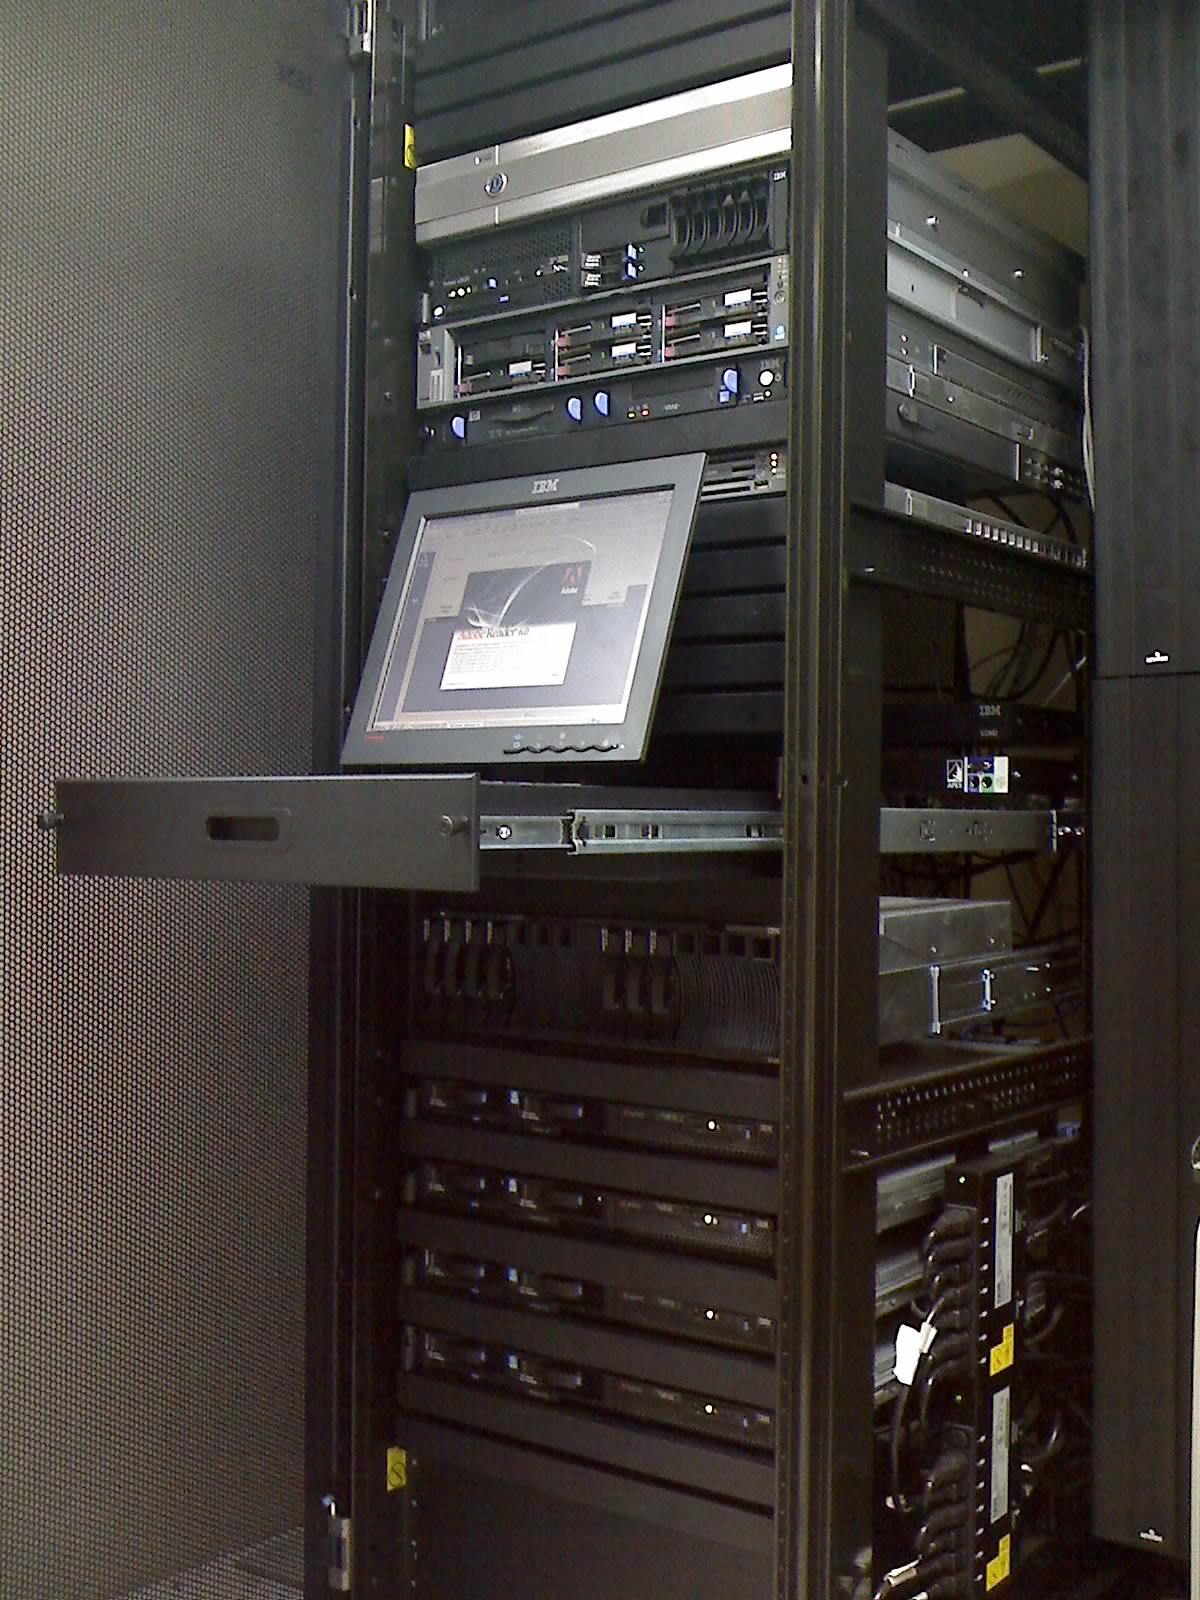
\includegraphics[width=0.75\linewidth]{Wiki_Rack001.jpg}
	\caption{Foto van Jfreyre afkomstig van \url{https://commons.wikimedia.org/wiki/File:Rack001.jpg}}
\centering
\end{figure}

Om hogere dichtheden te bereiken wordt er gebruik gemaakt van blade servers\index{Blade servers}. Bij blade servers zitten er meedere servers (blades) in \'e\'en fysieke behuizing (19''-kast). De servers delen een backplane, de voeding(en) en de behuizing waardoor er effectief meer servers passen op dezelfde oppervlakte. Een nadeel van blades is dat de warmte ontwikkeling ook veel meer geconcentreerd wordt en dat kan leiden tot zogenaamde hotspots, wat slecht is voor de koeling.

\section{Stroomvoorziening}
Het aansluiten van de servers gebeurt zoveel mogelijk in het cabinet, zodat de kast een gesloten geheel vormt. De spanning voor de servers wordt aangeboden via een PDU (Power Distribution Unit). Een PDU is vergelijkbaar met een verdeeldoos in het dagelijksgebruik. De aansluingen zijn vaak anders. De meest gebruikte aansluit stekkers zijn de C13/C14 stekkers:
\begin{figure}
\end{figure}

Een extra functie die je tegen kan komen in de PDUs is de mogelijkheid om elke uitgang te schakelen via bijvoorbeeld het netwerk (switched PDU). Via een remote protocol zoals bijvoorbeeld een web-interface of ssh kan je inloggen op de PDU en de spanning naar een socket schakelen. Op deze manier kan je een server die niet meer reageert op afstand herstarten in de hoop dat deze na een herstart weer op afstand bedient kan worden. Zo niet dan moet je toch naar de serverruimte lopen.

Een andere functie die je op PDUs kan aantreffen is een verbruiksmeter (metered PDU). Sommige PDUs meter alleen het totale verbruik van de aangesloten apparaten, andere varianten kunnen per socket meten hoeveel het verbruik is. Op deze manier kan je bijvoorbeeld het verbruik doorbelasten naar de gebruiker.

\section{Netwerkbekabeling}
De meeste kasten hebben in de kast een plek waar de servers aangesloten kunnen worden op het netwerk. De traditionele manier is dat een kast voorzien is van een patchpaneel. In het volgende hoofdstuk zullen we ook ander oplossingen bekijken. De servers worden met zogenaamde patchkabels (flexibele kabels) aangesloten op het patchpaneel. Om de koeling in de kast niet te veel te verstoren is het van belang dat de kabels op een ordelijke manier in de kast verwerkt worden en het geen spaghetti wordt.

Om de kabels netjes weg te werken zitten er horizontale kabel begeleiders in de kast om de bekabeling van de servers naar de zijkant te brengen en er zijn vertikale kabelbegeleiders die de kabels begeleiden van boven naar beneden of van beneden naar boven.

De patchpanelen zijn bekabeld met stugge (solide) kabels die de kast verbindt met de rest van de serverruimte.


\chapter{Netwerk voorzieningen}
\section{Hi\"erarchisch Netwerk Ontwerp}
Het Hi\"erarchisch Netwerk Ontwerp is een oorspronkelijk door Cisco bedacht model. Dit netwerk model bestaat uit 3 lagen. De access laag, de distributie laag en de core laag zoals weergegeven in figuur \ref{HND}.

\begin{figure}[H]
\centering
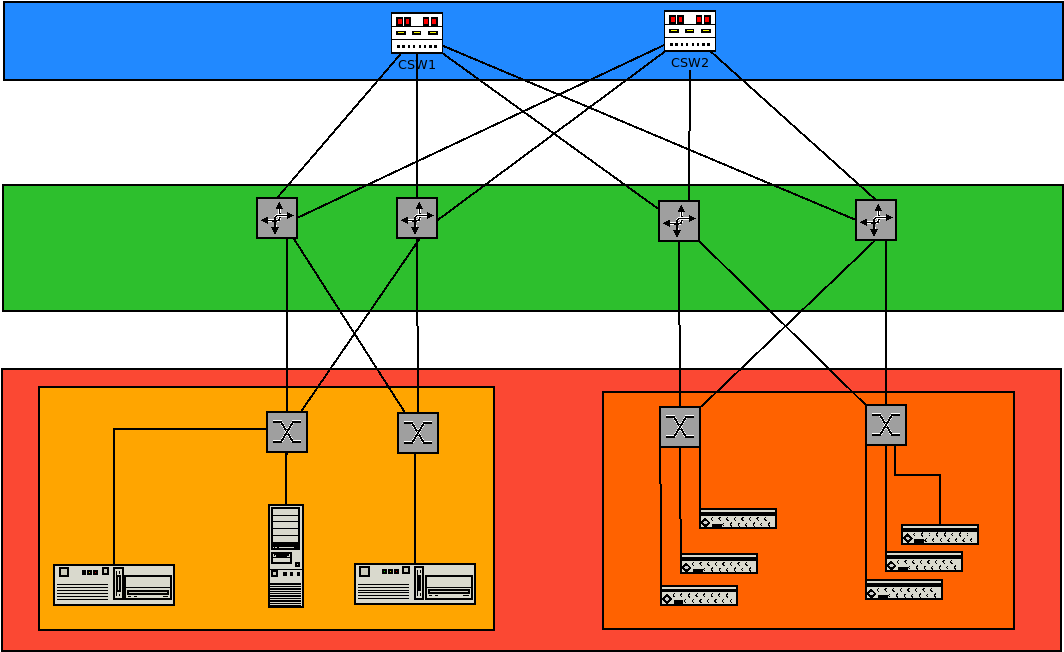
\includegraphics[width=\linewidth]{HND.png}
\caption{Blauw is de core, groen is de distributie laag en rood is de access laag met links de gebruikers en rechts der servers}
\label{HND}
\end{figure}

Op de access laag worden over het algemeen access switches gebruikt (OSI-layer 2), maar ook routers kunnen op deze laag voorkomen. Dit zijn "goedkope" switches die zorgen dat er voldoende poorten zijn voor alle gebruikers en alle servers in het netwerk. VLANs worden vaak op de access laag gebruikt om broadcast domains van elkaar te scheiden. De kosten per port is hier vaak de belangrijkste afweging. Het uitvallen van een access switch treft alleen de aangesloten gebruikers en heeft verder geen invloed op de rest van de organisatie. Dit is niet het geval als het een access switch in de serverruimte is waar meerdere servers aan hangen.

Op de distributie laag vinden we de meer intelligente devices die bijvoorbeeld afdelingen binnen een organisatie van elkaar scheiden door bijvoorbeeld firewalling, IP-routing en filtering. Ook QoS wordt op vaak op deze laag geregeld. Verbindingen naar andere kantoren van een organisatie behoren ook tot de distributie laag. 

De core laag bevat vaak de duurste netwerk onderdelen omdat deze moeten zorgen dat er grote hoeveelheiden data op een snelle manier verdeeld worden over de verschillende distributie componenten. Vaak zijn de core componenten redundant uitgevoerd. De hoogste netwerksnelheden per port vinden we vaak in deze laag. Omdat snelheid hier de fundamentele factor is vind hier geen of nauwelijks filtering plaats. Op deze laag kunnen we switches of routes (Layer 2 of 3 technologie) tegen komen.


\section{Patch-panelen}
Patchpanelen zijn passieve componenten, dat betekent dat ze niet iets met het signaal doen. Patchpanelen worden veelal in serverkasten gebruikt om de servers met patchkabels te koppelen aan de bekabeling die naar de serverruimte switches lopen. De IEEE 802.3 ethernet standaard zegt dat de maximale lengte van een ethernet kabel 100 meter is waarbij er twee keer 5 meter patch kabel gebruikt mag worden en dat de overige 90 meter moet bestaan uit solide koper bekabeling. Deze solide koperbekabeling wordt dan ook vaak gebruikt als bekabeling tussen een patchpaneel en de switch waarbij binnen de kast gebruik gemaakt wordt patchkabels die bestaan uit stranded (getwijnde) bekabeling.

Patchpanelen kunnen bovenin of onderin de kast gemonteerd worden, of in het midden van de kast. Het voordeel van de montage in het midden van de kast is er minder verschillende kabellengtes nodig zijn om de servers aan te sluiten op de patchpanelen en dat de kabelbomen aan de zijkanten van de kast kleiner zullen zijn omdat de ene helft omhoog loopt en de andere helft maar beneden. Dit helpt in het overzichtelijk en netjes houden van de bekabeling in de kast.

Patchpanel montage:
\url{https://spl-play.learningcloud.me/admin/sprints/5e3b1e8e79a83f25dd79f792/}

Patchbekabeling:
\url{https://spl-play.learningcloud.me/admin/sprints/5e3b1eea32eea20fcd021bb7/}


\section{Top of Rack Switches}
De zogenaamde "top of rack"-switches vervangen de patchpanelen in een kast. Een "top of rack"-switch kan natuurlijk ook in het midden of onderin de kast hangen. Het voordeel van een switch inplaats van een patchpaneel is de verminderde hoeveelheid bekabeling van het rack naar de serverruimte switch. Het nadeel is dat de kabel van het rack naar de serverruimte switch alle data moet kunnen verwerken van alle servers in het rack.

\section{Netwerk bekabeling}
\index{Bekabeling}De bekabeling in een datacenter bestaat uit lange koperkabels, tot 90 meter, of fiber kabels die de verschillende componenten met elkaar verbinden. Deze zelfde kabeltypes worden ook gebruikt om verschillende datacentra onderling te koppelen. We spreken hier van de horizontale bekabeling door gebouwen, het zijn ook de kabels die lopen vanaf de switches naar de wall-oulets in de verschillende kantoren.

Naast deze horizontale bekabeling zijn er de patchkabels die switches of patchpanelen verbinden met servers of patchpanelen met de de poorten van switches. Het zijn de flexibele kabels die makkelijk verlegt kunnen worden.

De kabels in een datacentrum kunnen worden weggewerkt onder de vloer, boven een systeemplafond of in metale kabelgoten die aan het plafond hangen.


\chapter{Voeding}
Het aansluiten van een datacentrum op het elektriciteitsnet in Nederland gebeurd meestal met 10 kVac of 20 kVac aansluitingen. Transformatoren zetten de aangeleverde hoogspanning om in 400 Vac welke de binnenkomende spanning is voor het datacentrum. Dit is de ingangsspanning voor de Main Distribution Boards (MDBs)\index{MDB}\index{Main Distribution Board}. MDBs zijn panelen of kasten die de zekeringen, schakelaars en aardlekzekeringen bevatten. De MDBs distribueren de spanning naar de verschillende onderdelen zoals UPS (Uninterrupted Power Supply)\index{UPS}\index{Uninterruptable Power Supply} systemen. Uiteindelijk wordt er dan 240 Vac naar de 19"-kasten gestuurd.

Het starten van de generator(en) is meestal een taak van de MDBs, deze doen dat zodra ze het wegvallen van het elektriciteitsnet waarnemen.


\section{Electriciteitsnet}
Een redundant systeem heeft twee aanvoerleidingen vanuit het elektriciteitsnet, het liefst vanuit een verschillende richting of van verschillende leveranciers. Dit zorgt ervoor dat er spanning blijft ook als \'e\'en aanvoerlijn uitvalt. Daarmee zijn we nog niet veilig want ook het totale elektriciteitsnet kan uitvallen en dan zit het datacentrum alsnog zonder spanning. Om dat op te kunnen vangen worden er vaak generatoren geplaatst bij een datacentrum. De generatoren werken op diesel of gas en wekken elektriciteit op dat voldoende is om een datacentrum voor bijvoorbeeld 24 of 48 uur van spanning te voorzien. Het opstarten van generatoren kost echter tijd, we laten ze niet dag en nacht draaien dat zou te veel energie (diesel of gas) kosten. De overbrugging tussen het uitvallen van het electriciteitsnet en het opstarten van de generator wordt opgevangen door een UPS.


\section{UPS}
De functie van de UPS is tweeledig. De eerste taak is het opvangen van kleine pieken en dalen in de elektriciteitsvoorziening. Computer apparatuur is over het algemeen gevoelig voor spanningswisselingen. Door de aanvoer eerst door een UPS systeem te laten gaan werken zorgen de batterijen van de UPS voor demping van pieken of opvulling van dalen waardoor er een veel gelijkmatigere aanvoer van vermogen is. De tweede functie van de UPS is het opvangen van de periode tussen het uitvallen van het elektriciteitsnet en het starten van de generator. Over het algemeen moet een UPS systeem het gehele datacentrum voor ongeveer 5 minuten van het volledige vermogen kunnen voorzien, zodat de generator de tijd heeft om meerdere keren te starten. Ook hier moet rekening gehouden worden met het feit dat de generator misschien niet meteen de eerste keer start.

UPS systemen zijn traditioneel gebouwd met batterijen, modernere varianten hebben een vliegwiel.

\url{https://download.schneider-electric.com/files?p_File_Name=DBOY-77FNCT_R2_EN.pdf&p_Doc_Ref=SPD_DBOY-77FNCT_EN}

\subsection{Batterijen}
Traditioneel gebruiken de meeste uninterruptable power supply systemen batterijen. Batterijen kunnen relatief makkelijk veel energie opslaan, het nadeel is dat ze veel onderhoud vergen en regelmatig gecontrolleerd moeten worden op hun functioneren.

Batterijen zijn DC (Direct Current) spanningscomponenten, de aanvoer is AC (Alternating Current) en ook de levering aan de cabinetten is een wisselspanning. Om als buffer te kunnen dienen moet eerst de aanvoer omgezet worden in DC en daar na moet de DC spanning weer omgevormd worden naar AC. De technieken voor een energiezuinige UPS halen een rendement van rond de 95\% of iets meer. Er blijven dus verliezen optreden en dus ontstaat er ook warmte.

\url{https://www.youtube.com/watch?v=UMtftcKACRA}



\subsection{Vliegwiel}
\index{UPS!Vliegwiel}\index{Vliegwiel}Het vliegwiel is geen nieuwe techniek, maar wel als functie in het datacenter. Veel serverruimtes maken nog gebruik van batterijen om voor langere tijd energie op te slaan. Een vliegwiel maakt gebruik van de traagheid van massa. De inkomende energie van het elektriciteitsnet zorgt ervoor dat een zware schijf rondgedraaid wordt, deze schijf is ook verbonden met een generator. Als de netspanning wegvalt zal het draaiende gewicht de generator laten doordraaien en zo kan ongeveer 15 seconden tot een minuut aan spanningsdip opgevangen worden. In die 15 seconden moet een dieselgenerator of gasturbine gestart worden die de wegvallende netspanning opvangt.

\url{https://www.youtube.com/watch?v=kQirOFEygJQ}

\section{Generator}
Een generator voor een datacenter is meestal een diesel of gas gestookte generator. Een generator is feitelijk een grote motor die elektriciteit opwekt. Het opstarten van een generator heeft enige tijd nodig waardoor er de noodzaak van een UPS blijft om de eerste klap op te vangen van het wegvallen van het elektriciteitsnet. De UPS kan wel kleiner zijn omdat deze alleen de directe dip hoeft op te vangen. Zodra de generator draait heeft de UPS geen functie meer.

Bij de grotere datacentra kunnen generatoren 24 tot 48 uur de spanning opvangen voordat ze zonder brandstof zitten.

\section{Distributie paneel}
\index{MDB}\index{Main Distribution Board}De Main Distribution Board of in het Nederlands het Distibutie Paneel\index{Distributie Paneel} is een stuk elektronica in een datacentrum dat de inkomende spanning distribueert, als het nodig is transformeert, bewaakt en monitort. Op een MDB kom je zekeringen, aardlekschakelaars, hoofdschakelaars en meters tegen. De zekeringen en aardlekschakelaars kunnen bij overbelasting of een aardlek lijnen afschakelen. De meters geven weer wat de spanning is en wat het huidige stroomverbruik is.

MDBs zijn goed te vergelijken met de functionaliteit van de meterkast in een huis.


\chapter{Koeling}
Vroeger was het grootste probleem in een datacenter de ruimte, het snel groeiende aantal servers stuite op een ruimte probleem. Met de opkomst van virtualisatie is dat probleem getackeld. De virtualisatie cre\"eerde echter wel een ander probleem: koeling. 10 servers die hoofdzakelijk uit hun neus staan te peuteren verbruiken stroom, maar cre\"eeren nauwelijks warmte. E\'en server die stevig staat te stampen om 10 virtuele machines in de lucht te houden gebruikt minder stroom dan de tien bij elkaar opgeteld, maar zorgt voor meer warmte dan de 10 machines bij elkaar.

De warmte die veroorzaakt wordt door de servers in het datacenter moet worden afgevoerd. Traditioneel gebeurde dat met airco's, maar met de ontwikkeling van groenere datacentra wordt er steeds vaker voor andere technieken gekozen, zoals het koelen met buitenlucht of het koelen met vloeistoffen.


\section{Lucht circulatie}
De traditionele manier van koelen koelt de gehele serverruimte. De koude lucht wordt onder de verhoogde vloer ingebracht, komt via roosters in de koude corridor tussen de servers (aan de voorkant van de servers), de servers zuigen de lucht aan de voorkant aan via hun ventilatoren en blazen de warme lucht er aan de achterkant uit in de warme corridoor tussen de serverracks. Ventilatoren aan het plafond (warme lucht stijgt op) voeren de warme lucht af.

\url{https://www.youtube.com/watch?v=xBxyhxmhigc}


\section{Temperatuur}
Elektronica werkt het best bij temperaturen van 20 tot 22 graden Celcius, echter elke graad Celcius temperatuur verhoging maakt dat we minder stroom verbruiken om te koelen. Daarom worden veel datacentra op 25\textdegree C gehouden.


\section{Luchtvochtigheid}
\index{Luchtvochtigheid}\index{Datacenter!Luchtvochtigheid}Ook de luchtvochtigheid is van belang zie hiervoor een artikel van bit.nl: \url{https://www.bit.nl/news/88/468/De-zin-en-onzin-van-luchtbevochtiging}


\section{Koeltechnieken}
\subsection{Compressorkoeling}
\index{Compressor}\index{Airco}\index{Koeling!Airco}Compressor koeling ook wel de airco (air compressor) genoemd is de klassieke manier om datacenters te koelen. Het systeem werkt op basis van water. Warm water wordt naar een unit gebracht die buiten hangt of staat. De koude lucht koelt het water af en het koude water wordt weer naar binnen gepompt om de warme lucht uit de serverruimte te koelen. Als het water niet voldoende afkoelt aan de buitenlucht worden er compressorkoelers gebruikt om het water verder af te koelen.

Het nadeel van dit systeem is dat er dure compressors in zitten en pompen en dat het geheel zelf behoorlijk wat stroom verbruikt. Daarnaast geldt ook hier, hoe meer onderdelen hoe meer kans op defecten.

\subsection{Adiabatische koeling}
Bij adiabatische koeling\index{adiabatische koeling} wordt de warme lucht uit de serverruimte gekoeld door koelers in de buitenlucht te besprenkelen met water waardoor verdamping optreedt. Dit kost natuurlijk water wat niet erg milieu vriendelijk is.

Een alternatief is de indirecte adiabatische koeling\index{indirecte adiabatische koeling}\index{adiabatische koeling!indirect}. Via een warmte wisselaar wordt de warme lucht direct gekoeld aan de buitenlucht, als de buitenlucht te warm is om voldoende te koelen dat wordt er teruggevallen op het gebruik van de verdamping van water voor de koeling. Voordeel van dit systeem is dat er geen buitenlucht in het datacenter terecht komt.

\subsection{PCM koeling}
PCM\index{PCM} staat voor Phase Change Material\index{Phase Change Material}. De techniek gebruikt de overgang van vast naar vloeibaar en van vloeibaar naar vast om kou of warmte op te slaan en werkt dus feitelijk als een thermische batterij.

De PCM techniek maakt gebruik van de buitenlucht en het feit dat de temperatuur 's nachts lager is dan overdag. Een anorganische stof wordt door menging met zouten zo ingeregeld dat deze vanaf een bepaalde temperatuur stolt of smelt. De warmte uit de serverruimte zal overdag de stof doen smelten hierdoor kan de PCM grote hoeveelheden warmte opnemen. Als de buitenlucht beneden de ingestelde temperatuur komt dan kan de buitenlucht de opgeslagen warmte afvoeren waardoor de stof weer stolt.

Deze techniek gebruikt aanmerkelijk minder stroom dan een traditionele airco-koeling. Fabrikanten claimen tot 90\% vermindering van het energieverbruik.

\subsection{Vloeistofkoeling}
Een techniek die langzaamaan ingang lijkt te vinden in het datacenter is het gebruik van vloeistofkoeling. Het is een techniek die gamers al wat langer kennen, maar die beperkt bleef tot thuis gebruik. Sinds kort wordt deze techniek ook gebruikt voor servers in de sreverruimte. De techniek komen we vooral tegen bij HPC (High Performance Computing) clusters.


\chapter{Beveiliging}
\section{Redundantie}
\index{Redundantie}Datacenter redundantie kan op verschillende manieren worden uitgedrukt. Om een 100\% uptime te bewerkstelligen is het noodzakelijk om voeding en koeling redundant uit te voeren. Als bijvoorbeeld een koelunit ermee stopt moet er voldoende extra koelcapaciteit zijn om de koeling van de defecte unit over te nemen.

Bij een volledig belast datacenter zonder defecten wordt de redundantie uitgedrukt als N\index{N}\index{Redundantie!N}. Dat wil zeggen geen redundantie. Zodra er een calamiteit is is er geen overcapaciteit om dit op te vangen en zal er dus downtime optreden.

\subsection{N+1}
Minimale redundantie wordt verkregen met N+1. Door bijvoorbeeld een compleet redundant UPS systeem neer te zetten kunnen we onderhoud uitvoeren op 1 UPS, de andere UPS kan dan de volledige load op zich nemen mocht er een stroomuitval zijn tijdens het onderhoud.

Een algemene regel bij het ontwerpen van datacentra met een N+1 regel is dat voor elke 4 units die we nodig hebben we 1 extra unit plaatsen. Dus als er in een ruimte 8 koelunits nodig zijn dan plaatsen we er 10.

\subsection{2N}
\index{2N}\index{Redundantie!2N}Een volledig redundant systeem heet 2N, dit betekent dat voor elke unit we plaatsen er een redundante unit geplaatst wordt. Als er 8 koelunits nodig zijn, dan plaatsen we er 16.

\subsection{2(N+1)}
Is een volledig redundant systeem van een N+1 opstelling. Dit geeft de zekerheid dat zelfs als een volledig systeem eruit ligt er nog steeds N+1 redundantie is. Het nadeel is natuurlijk wel de hoge kosten, zowel qua aanschaf als qua onderhoud, en de vele extra vierkantenmeters die nodig zijn voor alle extra units.

\subsection{xN/y}
\index{xNy}\index{Redundantie!xNy}Een variant op de 2N oplossing is een oplossing waarbij de lasten verdeeld worden. Stel we hebben een serverrack dat 1500 Watt nodig heeft bij totale belasting. Als we dat redundant willen maken met 2(N+1) betekent dat dat we 2x 1500 Watt UPS nodig hebben voor N+1 en dat moeten we verdubbelen voor 2x N+1, dus we hebben 4x een 1500 Watt UPS systeem nodig.

Door de lasten te verdelen kunnen we een soortgelijke bescherming krijgen tegen lagere kosten. Door de last te verdelen over bijvoorbeeld 3 systemen van 750 Watt zouden we bij uitval van 1 systeem een capaciteit van 1500 Watt over. We hebben dan dus 3 systemen, kleinere en goedkopere systemen, waarvan er 1 volledig mag uitvallen (2 blijven er werken). Dat noemen we \index{Redundantie!3N/2}3N/2. Voor de berekening van de capaciteit per systeem nemen we de totale capaciteit die we nodig hebben (N) en delen dat door het aantal systemen dat moet blijven functioneren (y). In dit voorbeeld dus 1500/2 = 750 Watt. Voor de redundatie hebben we 1 systeem nodig en daarmee komt het totaal aantal systemen (x) op 3.

Met \index{Redundantie!4N/3}4N/3 hebben we 4 systemen waarvan er 1 mag uitvallen. Uit ons vorige voorbeeld zou dat betekenen dat we 4 UPSen van 500 Watt (1500/3) neerzetten waarvan er 1 mag uitvallen zodat we dan nog steeds 1500 Watt over houden. 4N/2 geeft ons 4 UPSen van 750 watt waarvan er 2 mogen uitvallen.

\section{Toegangsbeveiliging}
Afhankelijk van de grootte en de locatie van een datacentrum kunnen er verschillende toegangsbeperkingen zijn. Een kleine ruimte kan afgesloten zijn met een sleutel of een paslezer, de grote datacentra hebben een poort, toegangscontrole met paspoort controle en afgesloten kasten zodat je alleen bij jouw kast kan komen. Elke colo (colocatie) heeft zijn eigen procedures voor toegang, waarbij alleen toegang op afspraak de meest bekende is. Ook wordt er geregistreerd wie er binnen is zodat in geval van een calamiteit of een latere controle vast te stellen is wie er in het pand aanwezig was.

Vele datacentra zijn tevens uitgerust met camera's, infrorood censoren en andere detectie en monitoring middelen.

\section{Calamiteiten bewaking en beveiliging}
Daar er in een datacentrum veel servers hangen is het grootste risico oververhitting van kabels en het daardoor onstaan van brand. Blussen met water is in een ruimte met zoveel stroomvoorzieningen niet verstandig, blussen met poederblussers betekent dat je daarna de servers weg kan gooien om de elektrische componenten aangetast worden, dus de beste manier om een serverruimte te blussen is door de zuurstof weg te halen. Een datacentrum wordt bij brand dan ook vaak volgepompt met bijvoorbeeld CO2.


\chapter{Onderhoud}
% Koeling
% Batterijen
% Stof
% Blusmiddelen
% 1x per jaar controle elektriciteit (noodstroomtest)

\chapter{TCO}\index{TCO}\index{Total Cost of Ownership}
% Boekjes virt TCO
% Boek Security in systemen en netwerken MTBF
% highavailability en scalability???
% Voordelen outsourcen
% Nadelen outsourcen (opdracht?)

%%%%%%%%%%%%%%%%%%%%%
%%% Index and End %%%
%%%%%%%%%%%%%%%%%%%%%
%\backmatter
\printindex
\end{document}

%%% Last line %%%
